% Todo:

\documentclass[12pt]{report}
\usepackage{hyperref}
\usepackage[no-math]{fontspec}
\usepackage{xeCJK}
%\setCJKmainfont{KaiTi}
%\setCJKmainfont{SimSun}
\setCJKmainfont[BoldFont=KaiTi,ItalicFont=SimHei]{KaiTi}
% \setCJKsansfont{SimHei}
% \setCJKmonofont{SimKai}
% \setmainfont{Arial}

\usepackage{cite}
\usepackage{graphicx}
\usepackage{float}
\usepackage{amsfonts}
% \usepackage{amsmath}	% for \tag
\usepackage{amssymb}	% for \multimap
% \usepackage{stmaryrd}
\usepackage{color}
%\usepackage[square,numbers]{natbib}
%\nocopyright
%\usepackage{latexsym,amsmath,amssymb,graphicx,hyperref}
%\usepackage{times} % gives you a bit more space if needed
\usepackage{titlesec}		% change color of section headings
\usepackage{verbatim}
\usepackage{pdfpages}		% book cover
\usepackage{framed}			% title page's box
\usepackage{datenumber,fp}	% for year calculations
\usepackage{accents}		% for dots under Chinese for empahsis
\usepackage[nohints]{minitoc}		% mini table of contents

\titleformat{\chapter}
{\color{blue}\normalfont\huge}
{\color{blue}\thechapter\\}{1em}{\flushleft}

\titleformat{\section}
{\color{blue}\normalfont\large\bfseries}
{\color{blue}\thesection}{1em}{}

\definecolor{Magenta}{rgb}{0.4,0.1,0.4}  % Magenta
% \definecolor{LogicColor}{rgb}{0,0,0}	% for black-and-white paper

\newcommand{\tab}{\hspace*{1cm}}
\newcommand{\concept}[1]{\textbf{\textcolor{blue}{#1}}}
\renewcommand{\textbf}[1]{\textcolor{red}{#1}}

% Make dots under Chinese characters for emphasis
\renewcommand{\d}[1]{$\underaccent{\scalebox{0.4}{\textbullet}}{\textrm{#1}}$}
\makeatletter
\newcommand{\ds}[1]{%
  \@tfor\next:=#1\do{\d{\next}}}
\makeatother

\newcommand*\sadface{\includegraphics[scale=0.25]{face-sad.png}}
\newcommand*\smiley{
\includegraphics[scale=0.5]{smiley.jpg}}
%\newcommand*\vignette{\centering{\color{blue} --- \quad $\diamond$ \quad --- \quad $\diamond$ \quad --- \quad $\diamond$ \quad --- }\par}
\newcommand*\vignette{\begin{center}\color{blue}  --- \quad \S \quad --- \quad \S \quad --- \quad \S \quad --- \end{center}}

\setlength{\oddsidemargin}{0cm}
\setlength{\evensidemargin}{0cm}
\setlength{\textwidth}{16.5cm}
\linespread{1.3}

\begin{document}

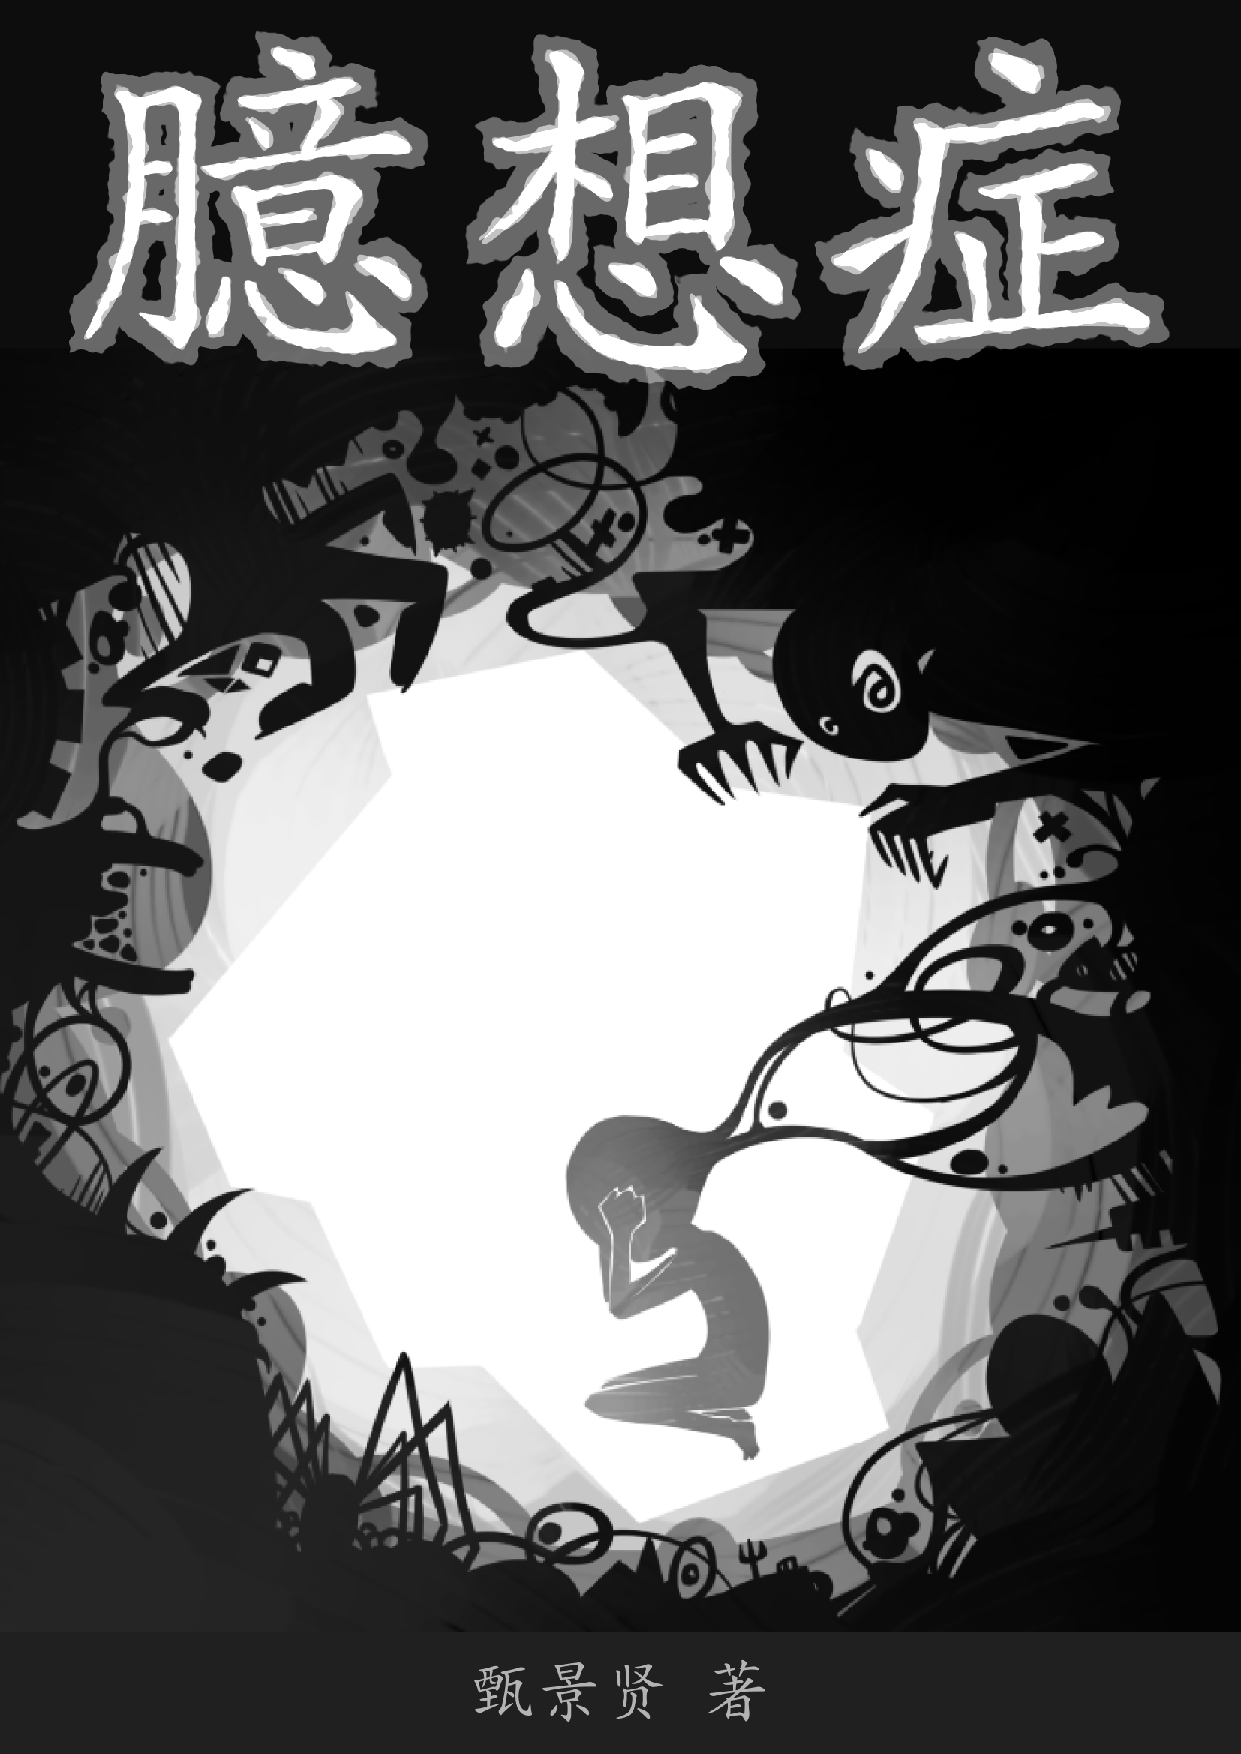
\includepdf{cover1}
\cleardoublepage
\title{\Huge{臆想症}}
\author{YKY (\textit{甄景贤})}
% \date{27 May 2015}
% \institute{}

% Calculation of some years
\newcounter{dateone}
\newcounter{datetwo}
\newcounter{datezero}

\setmydatenumber{dateone}{1991}{08}{01}		% Cousin visit HK in summer
\setmydatenumber{datetwo}{1996}{09}{01}		% first arrive in USA
\setmydatenumber{datezero}{\the\year}{\the\month}{\the\day}

\FPsub\resulta{\thedatezero}{\thedateone}
\FPdiv\resultb{\resulta}{365.2425}
\FPround\resultb{\resultb}{0}

\FPsub\resultc{\thedatezero}{\thedatetwo}
\FPdiv\resultd{\resultc}{365.2425}
\FPround\resultd{\resultd}{0}

\large

\tab\tab\tab \parbox{9cm}{\textit{Love is an act of endless forgiveness,\\
a tender look which becomes a habit}}
\vspace{0.5cm}
\begin{flushright}
\textemdash\, Peter Ustinov \hspace*{3cm}
\end{flushright}

{\let\newpage\relax\maketitle}

\maketitle
\setlength{\parindent}{0em}
\setlength{\parskip}{2.8ex plus0.8ex minus0.8ex}

\small

\begin{framed}
这篇文章的起源是回答《知乎 www.zhihu.com》网站的问题『精神分裂症患者眼中的世界是什么样的?』

很多地方写得不好,但我想尽快发表这个草稿,以后还会修改和添补。

欢迎你们提问或提供意见。

封面插图:  Nami-Tsuki, ``Paranoia or something'', DeviantArt.com
\end{framed}
\large

\dominitoc
\tableofcontents

\chapter{臆想症}

我有 paranoia (逼害臆想),特别地叫 Truman Show syndrome。 在《Truman Show》这部 1998 年的电影里,主角活在一齣真人表演里,他身边的人都是演员,但从小欺骗着他,最后他走出了这个骗局。 在外国有很多人有这种臆想,多到形成了症候群的名字。

我 25 岁时 (1996 年) 初到美国,那时迷恋我的美国堂妹但遭拒绝。 再加上在外国生活和很少朋友, 而且我从小便对白人的种族歧视很有反感,所以觉得自己活在充满敌意的环境里。 这些因素,令我到了美国不够一年便产生了 Truman Show 臆想。 (起初是怀疑有人偷看我的电邮开始....)

\resultb 年后的今天,我其实仍然未「康复」。 我现在打这篇文章,我的脑子一半觉得自己独自在房间里打字,一半觉得是在全世界 Truman Show 的众目睽睽下打字。

你可能觉得我疯了,为什么像 Truman Show 那样荒谬的情节,都会觉得是真的?

我正在研究人工智能,这个技术在不久将来可能会颠覆世界秩序。 例如,白人和有色人种的主要分别,可能只是外貌上的不同,但这外貌是由基因遗传的,我们中国人不能拥有那些基因,除非强抢他们的女人来交配。 有人工智能后,技术的发展可使人长生不老,那时候人类会脱离基因的约束,我们想变什么模样都可以。 而白种优势 (white supremacy) 也将会随之消失。

所以,西方人可能不想让中国人掌握这技术。 而我确实遇到了来自美国的人工智能研究者的排斥:他们叫 OpenCog,创始人是 Ben Goertzel,他现在颇有点名气,你可以上网查查。 我试过很多次想加入他们,但他们态度很不友善、诸多阻挠。

所以,如果我觉得美国或西方有人想害我,其机率实在未必是零。 你不见有很多反美的政治人物都被害死了? 而我的立场是坚决反对种族歧视,在逻辑上必然导致要反美。

故事太长了,想找个代笔的人,写本书在什么地方发表。 有兴趣可联络。

住过精神病院 3 星期,在那里见过一些人和事,很同情他们。 我被吓得半死,装着正常求他们放我,终於在圣诞节那天他们放了我出来,使我想起 《One Flew Over the Cuckoo's Nest》\footnote{《飞越疯人院》(1974)}这齣戏 (戏中的正常人被电击至白痴,而那以为自己是耶稣的人却成功逃离)。 戏中还教人把药藏在脷底下,想不到这点小知识后来对我很有用。

关於那些精神科药物,它们是没有帮助的,只是把神经传播的讯号分子阻碍 (blocking),会导致人嗜睡、没精神、失去动机 (motivation)、性欲等。 男孩子还会变女性化。 说得简单点就是用药物把脑部部份切除 (虽不是永久性的)。 我因为先前研究过如何将人脑的「意识」上载到电脑上 (mind uploading),所以对神经科学很熟悉。 信我吧!

甄景贤是真名 —— 为什么用真名? 因为我有一半认为,你们已经知道这一切了 \smiley

\chapter{殖民主义}

我爸以前在香港当皇家警察的,后来香港回归后他继续做了几年才退休。 我年轻时从没有因为父亲的职位觉得不妥,但到了美国后就开始强烈地意识到了。 毕竟,为殖民主义服务,是卖国的一种形式。 奇怪的是,在香港,大部分人压根儿不会想到殖民主义有何不妥。 有人甚至认英国政府是「契妈」、比生母还要亲。 为什么这样呢? 殖民时期的香港虽说是个「华洋杂处」的地方,但其实西人对华人来说,仍然是「高不可攀」的 (这情况或许正在改变),有很多香港人提到要讲英语便会脚软。 在这种恐惧之下,他们不能正确地认清殖民主义的真面目。

我接触美国后,有好几年都完全被他们的进步文明慑服了,就像小布殊说的 ``shock and awe'' 那样。 有时期连中式食物都不敢吃,要吃全西餐。 但后来回到香港,在报纸上看到「西方伪善\footnote{western hypocrisy}」这个术语,从此对国际间发生的事,真是豁然明白了很多。

小时,我有个阿姨,去了英国念文学。 我见她不多,印象中就只有一次她对我们忆述在英国念书的情景,说有一次集体用餐时,她伸手拿面包,有英国男生对她说 ``don't touch that bread!'' 那样的话。 (确切的那句话不记得了,总之是叫她不要碰那面包,应该不是叫她吃高纤面包吧?) 后来她在香港的一间 Islam 中学教书,得了白血病死了。 在我想像中,觉得她是个自尊心很强的人 (在外婆的女儿中,她大概是最漂亮的,学历也最高),因被人歧视而在郁结中死去。

\chapter{世界 A 和世界 B}

自从思觉失调之后,我无法分辨这个世界究竟是世界A (现实) 还是世界B (真人秀)。 在地铁看见别人窃窃私语时,不知道她们是不是在谈论我。 总觉得香港和美国的电视节目在含沙射影地嘲讽我,有时又用肥皂剧的角色映射我、咀咒我死掉; 这些都令我讨厌之极。 但我又无法分辨世界 A 和世界 B。 换言之,我已经变成了一个盲人,就像《圣经》里 Samson 和 Delilah 的故事:Samson 被她出卖之后,被人剪去头发和弄盲了,从此他的努力工作都是徒劳无功的,变成了他的敌人的笑柄。 (我是无神论者,但圣经里的故事有时是很有意思的。) 我常常觉得,我当初和堂妹的纠缠,就是解开这一切问题的关键,所以不停地分析那段日子。 那时候思想和感情都很混乱,是走上疯狂之路的开端。

首先要釐清的是,我虽然很迷恋她,但其实也看不起她、也有想要别的女孩,而我那时只不过是在海难中掉进了太平洋,像抓着救生圈那样缠着她不放。 因为她是 ABC\footnote{American born Chinese},她就像是一张打入白人社会的入场券,能娶到她该多好啊。 否则我就像漂浮在大海,徬徨着不能「上岸」。

终於在纽约见到她,她已经明显不喜欢我。 那时我带来了一本书,是一个加拿大华裔女孩写的,讲她离家出走后卖淫的自传式小说,我知道女孩子没有不喜欢那种书的,果然我把书遗在伯娘家,然后她两姊妹都看了。 书还回来后,竟然有堂妹的笔迹写的小纸条,就只一句 ``no escape except through death''\footnote{『没有出路,除非通过死』}。 那时我觉得她是在耸恿我去把我的某个中学朋友杀掉。 (因为堂妹最初跟伯娘到香港旅行,那是我最初喜欢她的时候,我把那中学朋友介绍给她,原以为大家可以一起开心玩,想不到他俩眉来眼去,把我变成傻子一样。) 我越来越觉得那是奇耻大辱,非要杀他报仇不可 (就像一把插在我和堂妹之间的剑,一定要拔掉),但自己又身陷真人秀里,怎能杀人? 而且,堂妹若真的爱我,怎会要我杀人为条件? 当初不是他俩在调情才做成这耻辱吗? 每想到这里就愤怒到浑身发抖。

十几年后,最近终於好像明白了她那句句子的意思。 其实在美国文化里,最高级的人是金发蓝眼的;如果红头发的话,是不祥的;如果黑头发,那么她们触摸的一切都会变成悲剧。 至於犹太人更不用说了,把卷曲的头发烫直再说吧。 而黄种人比犹太人更低级。 我妒忌我的美国堂妹比我「先上岸」,仿佛她先过我变成了白人,我妒忌到想把她杀了,而我以前从来未对人怀过那么深的怨恨。 而其实,这个所谓「上岸」指的是什么? 所有美国华侨,在美国只不过过着次等的、没有尊严、像影子一般的 existence。 就算 Whitney Houston\footnote{(1963-2012) 美国黑人女歌手,她的歌词里叫人要懂得自爱,不要活在别人的影子下,我中学时老师播给我们听。} 都不过是个影子,奥巴马更干脆背叛了自己黑人的那一半,他还 cool 到露出微笑。  注意:乔布斯\footnote{(1955-2011) 苹果电脑的创始人}就是一个「认继父母不认亲父母」的人。 在美国,有色人种越来越绝望,甚至当妓女贱卖,那些白人男孩都未必会揪一眼。 谁都上不了岸,我们在海难中互相拉扯,丑态百出。『除死以外没有出路』可能就是这个意思。

\chapter{American cousin}

1991 年(\resultb 年前),来自美国的伯娘和两个堂妹来香港旅游。 我 20 岁,刚进大学二年,堂妹 14 岁。

那时候家里很热闹,来自英国的表弟也和一个白人朋友来香港旅游,所有人都住在我家。  堂妹她们到达的那一晚,我刚从大学宿舍回来,她们已经进房睡了,妈在客厅中低声向我「汇报」描述这些新来的客人。    她面带愁容地说: 哎吔.... 那两个堂妹的打扮很「吓人」.... 那个大的痴肥,身体像座山那样; 那个小的,年纪轻轻已经涂指甲、口红、香水,像个「老人精」。   我听了之后心里已经很喜欢她; 这些故事从来就是这样开始的。

相识还不够一天,堂妹说:「堂兄妹也可以结婚,如果不生孩子的话。」 我故意面色很凝重地点头。

5 年后,痴情的我到纽约找她,她说她已有男友,她要结婚生孩子,我们不可能。 我和她纠缠,我说她不给我合理解释; 她说我像个 psychopath (精神病患者) 很可怖。 而我当时的确开始了被人监视的臆想 (她不知道); 我很想和她谈的原因之一就是想她帮我想清有没有被监视的问题 —— 甚至她也可能是观众之一?

其实 1991 年那暑假,初相识的几天之后,她已经换了态度,说:「我只想要个阿哥,把欺负我的人揍一顿。」 我当时的反应是:「Huh? 揍谁?」

\resultb 年来我不停思索为什么她嫌弃了我。

14 岁的她说:「(老)布殊在伊拉克打仗,他还一边打高尔夫球!」 我说我们香港人不问政事,不知什么叫打仗,与及一些类似的蠢话。  现在我明白到,她说的很对,她年纪小小已经很懂事。  现在我知道正确的答案是:「我要把 Uncle Sam 打到跪低,然后斩他的头下来!」

\vignette

在纽约的大学宿舍,正对着窗前是一颗大树,春天时,树上的一对鼬鼠 (?其实我也不清楚它是什么动物)天天在追逐,大概是发情期吧,那雄性的老是朝着雌性的尾部追去,但又总是追到贴近尾部 却又揽不住她,看起来就像只是为了嗅那气味,看得我直冒火。  我只身来到纽约,但堂妹不想见我,我们当时的处境分明就像那两只在追和被追的鼬鼠,我觉得那境象简直令人眼冤,就像拉粪和放屁的生理现象那样讨厌。  这令我想起一本小说的名字: The heart is a lonely hunter。  想起电影中理想的情侣,什么「青青珊瑚岛」、在花间嬉戏、女的含情脉脉地看着男的,那景象和我的现实截然不同。  我是在追者,她是在逃者,但青青珊瑚岛的他俩是两情相悦的。  一定有什么出错了,但又想不出是什么原因,感觉一切都和我作对,everything is against me。  莎士比亚说:世界是舞台,我们是演员,而我发觉我这「在追者」的角色是一个根本不可能演得好的角色。  我一步也不可以追,一追就错了,但我已经在追了。

我又想起一齣电影,年青人的漂亮妻子被敌人胖子看上了,他们互相比拼赌术,年青人把身家输光了,把妻子也拿来赌。  当然最后还是年青人赢了,在那结尾的一幕,他把妻子赢回,而胖子啕哭起来,那女的用手揉他的背 ~安慰他。  为什么这角色降临到我身上?

我又想起有一次在地铁里,有个母亲当着其他乘客的面在规教小女孩,而那小女孩用手掩着耳朵不听,似乎很懊恼她母亲把她的糗事公诸於世。  我觉得当时的我就是那小女孩,不想听到真相。

我心里产生一幅图像: 我没有穿衣服,黄色皮肤的身体像只低等动物,我很拙劣而原始地,用手捏着泥巴,在筑一道小围墙,想把堂妹围进去,而那围墙矮矮的细小得可怜,只够围着我自己一人,里面的环境污糟邋遢,而我堂妹居高临下看着我,我还懵然不知。  我越来越觉得这个围墙无法经营下去,真相像四面楚歌那样迫过来。  终於,我发觉堂妹在看我,我恼羞成怒,想骂她:『妳明知不会喜欢我,为什么不早点告诉我?』  然后又想起: 她岂不是一直反覆告诉我不喜欢我,而我却莫名其妙的听不进去?

我又想,所有人在成长的过程中都要经过失恋的痛苦,为什么我搞得特别糟糕?  很多旧同学也大学毕业了、结了婚、生了孩子,没听过他们闹出什么丑闻。  为什么别人适应良好,难道是母亲以前教漏了什么?   为什么教科书上没有?   也有一个旧同学,他在大学宿舍爬墙偷看女朋友的房间,发现她和另一男孩偷情,还摔下去跌断了腿。   他正是上面我提过的,和我堂妹眉来眼去那人。

有一晚在宿舍里,我鼓起勇气打电话给她,但又害怕,电话的听筒拿起了又放下,最后还是打了给她。 她问我『你想说什么?』   而我说:『我…… 我…… 我…… 』那样重复地口吃着那「我」字,真的有一兩分钟之久。  因为我觉得心虚,我不是真的爱她,而是因为得不到她,所以想征服她。  我觉得我对她的爱不是真的,我分明瞧不起她,但又很怕被她识破。  我不会为她而死,甚至我能肯定地预测到,如果追到她以后,我也会喜欢别的女孩。  那就像一场真心的比拼,而我心虚了,最后我说:『我 …… 我 …… 我 …… 很爱妳 。』  她好像觉得受了冒犯似的,挂断了电话。

我反覆思量,后来我在网上和一个美国女人谈起这件事,那女人态度有点傲慢,她说: ``So she's smart ...... Forget her and move on.''  

我想起,其实她似乎也喜欢很多男孩。 在她14岁那个夏天,我们不知怎地聊到性的话题。  我理所当然地说:「我喜欢很多种类的女孩,但妳是女孩,妳当然只会和妳真正喜欢的男生才做爱。」 可是她说:「不啊,我和谁都做。」 我被她突如其来的反驳搞得很不知所措,而且很害怕她会喜欢上别人。  当时我假设她说的这话不是真的,因为我不愿意相信。

等公车的时候不见公车,不等的时候却遇见很多。  在纽约单恋堂妹的时候,特别多女孩勾引我。 但我那时故意不睬别的女孩,以表示我对堂妹有多忠心。  其实那只是我一厢情愿地想找些理由逼她喜欢我。  在大学上课时,有个女生在后面丢了笔到地上,而我居然全身绷紧了不去帮她拾,因为我怕是她在勾引我。  我甚至隐约听到那女生很惊奇地低声说 ``what?'' 然后她自己拾回那笔。

\vignette

在纽约,她的 (不是男友的) 美国朋友 Ralph 对我动手动脚,警告我不要再骚扰堂妹。 我没有还手,当时的我实在搞不清发生什么回事。 然后我跟伯娘投诉堂妹为什么不给我解释,打了伯娘一下。 伯娘打电话招援,我被他们一众亲戚朋友打了一顿。 我说 Ralph 先动手打我,但我不知他们接收到没有。

被打一顿之后,我跌坐在房子外的草地上,手臂在流血(但只是皮外伤)。  伯娘指着我痛骂:「你这算是读什么书? 读屎片!?」 过后又写了张支票给我,也许是作为「失恋补偿」?  这次事件后我和她们很少见面了。

那天伯娘本来为了帮我搬家,特意从老远驾车到我住处,但我不感激她还觉得她们欠了我。 我那时处於人生的极低点,真是 inconsolable.

伯娘以前已经和我解释过:『她若真的喜欢你的话,不会是这样』、『你若不服气,将来努力点,胜过她。』 其实她的话很有道理,我听了之后真的很努力发奋。

\resultb 年后的今天,我看见那些软弱无能的香港人,有无法抑制的想朝他们面上揍一拳的冲动。 觉得不教训实在不成体统,但那岂不是等於打 \resultb 年前的我自己?

我妒忌堂妹,因她父母先到美国移民,她们很早便认识到外国人的 尔虞我诈 和 aggressiveness (侵略性),但外国也比我们进步很多,而我只是香港的驯良的乡下仔。 我很愤怒,为什么是个小丫头教训我,但我想不出有什么可批评她(除了一些琐事)。

但其实她也有缺点,也是个普通人。 14 岁的她也说过一些蠢话,蠢到笑死人。 想不想听? 例如她说 :「我以前不信有鬼,但看了《Ghost》\footnote{(1990)} 这齣电影后我真的信了。」 那个主演的 Patrick Swayze 现在真的变了鬼。

她又好像好心地告诫我:「千万不要信人!」 回想起来, 她的一句话,和我被那中学朋友出卖等事,真的令我什么人都不信了。 而彻底怀疑的结果就是我连所有人是不是在演戏都分不清,甚至包括她在内。

初相识的时候,我常为小事对她说「对不起」,但她说:「不要老是 say sorry,我最讨厌人说 sorry」,而我在她面前真的常常说错话或做错事。  她走之后我发了神经,无论什么情况都不对人道歉。  在纽约的大学,有一次迟到,理应对教授说 ``sorry I'm late'',但我却只说 ``I'm late''。 那教授很惊奇地说:「Mister Yan,你刚才对我说你迟到?」 我点了点头。 我其实很蠢,那大概是对堂妹的一种「无声的」投诉,『你看看我听你的话弄到什么地步?』 但在「世界 A」的解释下,教授和同学都不会听得懂,他们大概在纳闷:这中国人为什么不说 sorry?  然后必然想到帝国主义、种族歧视那些。

在纽约,她责备我为了见她而要我父母出钱供我到那里读大学,很「自私」。 但后来我憎厌她之后我又想:「我来美国读书有何不妥,纽约难道是你的?」 \ds{纽约是谁的}?

在宿舍的床上,我想着她,越想越觉得自己受骗了,但又说不出所以然。  突然间胸口觉得很闷,我用手臂锤了胸部一下,像打鼓那样,然后才意识到自己做了这个动作。  我立即心想:「妈的,怎么我这动作和猩猩一样?」  这下羞死了,看真人秀的所有观众一定笑到流眼泪。

\vignette

为了这件事,我父母飞来纽约调停,我们3人暂住在伯娘家的地库,堂妹她们就在楼上。 有一次我和妈妈独自谈话,她说堂妹把我寄给她那封情信给我爸妈看,还投诉我怎样骚扰她。 我对妈说: 我只是想听听堂妹的解释,和她谈一下(因为我想知道有没有人在监视我,那时我觉得全世界只有堂妹能明白我,而我不想和妈妈提到我患了被监视的病,因为她就是我要揭发的人之一),为什么她连跟我讲清楚也不肯呢.... 但我妈说:『我也问过她,但她说她不想见你。』  我说:『为什么她连和我谈一次也不肯呢....』 这句话未说完,我的眼泪不能控制地滚下来,像个小孩子地淘哭起来。 是我妈把我教成像大男人,她从小教我男孩子是不会哭的。

我哭了,实在想不到她怎会冷酷到这样.... 

我觉得被她出卖了....  她不会联合我对抗美国.... 而是她联合美国对抗我....

人们会逐渐忘记伊拉克战争.... 我会搞不清究竟有没有人在偷看我.... 别人会当我是疯子....

.... ....

过了很久,我才振作起来,叫自己不要相信那《圣经》Delilah 的故事,我不会被她出卖之后就完蛋了; 一个女人坏掉就换另一个。  但我真的至今也找不到一个好女孩。 

弟弟也从英国飞来美国探我,还陪同他的日本同学。 我还在骂堂妹「为什么不给我解释」,弟弟问我:『首先,你能不能接受她不喜欢你这件事?』  我说:『我当然可以接受她不喜欢我,我只是想她给我一个解释。』  弟弟说:『你这样做是``\ds{以己度人}'',你觉得分手必须解释清楚,但有些人就觉得什么也不说最好,你不能勉强她用你的方法....』 但我当时就是听不进去。 弟弟说,这次美国旅行,也因为我的事而蒙上阴影,令他对纽约留下很不愉快的印象。

我最近又记起,我问妈妈:『为什么她一句话也不能谈,妳不觉得很离谱?』 妈妈说:『有些女人就是这样的,她们喜欢将男人折磨和激怒,还这样引以为荣!』  我想起这话,觉得岂有此理,怎会好端端一个女孩有这种想法? 难道妳自己就是这种贱格女人?  噢.... 原来妳真的就是这样。

\vignette

我大伯早死,堂妹幼年丧父,她是那种没有管教的女孩,加上是美国人,常常笑我们老土,连我父母都怕了她的说话刻薄。 而我被父母管得透不过气,那使我很倾慕她。

在香港,我带她到一间叫 American Cafe 的地方饮咖啡,但她嫌那地方不是「正统」的美国餐馆 ,令我觉得很丢脸。 但其实,在香港吃麦当劳和吃一间非正统的美国餐厅,其可耻程度究竟有什么分别?

《红楼梦》\footnote{写於 1760s}里贾宝玉说男人都是污秽之物,但女人的本质是清纯的。 但据说第 80 回后不是曹雪芹所作,那么贾宝玉被骗婚、林黛玉殉情等情节,可能不是作者原旨。 而曹雪芹惯用的伎俩,不就是把读者引入陷阱,然后再将之幻象破灭 (disillusion)? 所以红楼梦才叫「梦」,不是吗? 我自己写作也喜欢这技俩! 但贾宝玉丢失了玉、和贾宝玉遇见甄宝玉等桥段,又像是神来之笔,后人续写会不会有那么好的想像力?

但其实都不用太追究了,因为那只是小说,而我的目的不是写小说,而是要进行客观的分析和计算。 所以我对所有人都批评,包括我自己。 我们要靠自己思考去找答案而不是尽信书。 据说 Fermat 也不知道 Fermat's Last Theorem 的证明,数学家一般认为他搞错了,真正的证明是要用到 20 世纪的数学。

像村上春树说,写作的确是一种自我治疗,因为不写出来的话连自己都搞不清谁是谁非。 我曾经恼怒到想杀掉堂妹,现在我只想分析清楚究竟是谁错了。 她绝对有自由拒绝我,也许是因为窘逼说不出口。 毕竟我们的 DNA 有 12.5\% 相同,大概她说不出口『哥哥,你又样衰又没本事,又老过我很多,所以我正式甩掉你 』? 现在我也常常不睬别的女人,例如那些不够漂亮、或不够聪明的。

堂妹其实也不算很漂亮,其实我在美国时有一个意识就是:如果连她都追不到,那些金发碧眼的妞儿就更加追不到了。 那使我惭愧,因为我只想像亨利 8 世那样娶 6 个老婆。 现在我也变得很滥交。 谁不会?  所谓用情专一 (monogamy) 只不过是年轻男女为了抬高身价,把自己卖得贵一点,之后又哭着说「对不起,我控制不了。」

但我始终很惭愧我当时觉得她不够白人女孩漂亮,想起她「嬲爆爆」(发怒时) 的脸。 我现在觉得中国女人很美,可能那才真的是精神错乱了 \smiley

\chapter{监视下的日常生活}

或者描述一下长期活在真人秀里是一种怎样的感觉。 

被堂妹和亲戚打了一顿之后,我肯定堂妹不喜欢我了,於是我名正言顺地可以开始追求新对象,我想到那些美国大学的女孩很漂亮性感,甚至咀角泛起了一丝微笑。  原本就不是很瞧得起这个身材胖胖矮矮的穷家女,失去了她又怎知不是福气?  这样想著,我走出大学宿舍到饭堂吃晚饭,在电梯内遇见两个金发的漂亮女生,她们在谈话。 美国有些女孩谈话时语气很特别,就算她们在说些无聊琐事,也好像你们男生应份要对她们关注。 其中一个女孩语气有点浮夸地说: ``I think he's such an \textit{asshole},'' 似乎在谈论她们认识的一个男生。  但我却似乎很明显地感觉到这话是冲著我来説的,因为我堂妹不是不喜欢我,她掴我是因为我的爱是假的,而我顺势放弃了她另结新欢了。 我很卑鄙.... 是吗?

\vignette

有次暑假从美国回来,探望嫲嫲,她喜欢在她家开著电视机。 我听到电视剧里的一句对白。  我自己从来不看电视,完全不知道是哪齣电视剧,也不知上下文,就只听到一个男的声音说:『唉,他们两个都这么卑劣,真是天造地设的一对!』  我立即觉得他们是在映射我和堂妹,心里很厌恶:「难道你们偷看我,就不卑劣?」  然后又想: 为什么觉得他们在说我呢?  这岂不是「对号入座」?

这样的感觉几乎每天也有,只要听到或看到别人的閒言閒语或任何琐碎的事,都会联想到是在映射自己。 

有时在家里自言自语,说了特别好笑的笑话,又会沾沾自喜,觉得全世界的女孩都听到了我聪明的笑话。

但当有些瘀事发生,则又会非常愤怒,因为我从来没有默许过这种监视,觉得全世界都在欺骗我,他们始终有一天要赔偿的。

\vignette

有些事情很巧合,无法解释。  刚从美国回来,那时我仍是特别喜欢白人女人,有一天在网上看到一个欧洲贵族的公主,她接受访问,头上戴了头箍很清纯可爱。  我想起来,实在很多年未见过女人戴头箍了,似乎这年代已经不流行。  然后我又觉得自己能在真人秀里间接地「结识」这位欧洲贵族,在沾沾自喜。

那时家里有个印尼籍的傭人,她的样子也很漂亮,但可能是主仆的关系,我觉得她老是跟我作对,令我很烦厌。 奇怪的是,我在网上看到那欧洲公主的第二天,那印傭女孩又「跟风」戴了头箍出现。 我那时期正和她闹得很不愉快,看到她头上的头箍,顿时产生厌恶,因为那就像是对我说:『你不喜欢我吗?那我也要破坏你和欧洲公主的好事。』

回想起来,其实那印傭天天换发饰,另一天她又变成 dreadlocks,所以有一天戴了头箍也不足为怪啊。

\vignette

最近有一次,认识了一个大陆的女朋友,我告诉她我接近中年以后比较少运动了,清洁家居就是我的运动。 然后我们在家看电视,那天是愚人节,我们看到一种很奇怪的运动项目,叫「冰壶」,但看起来就像有个机械人吸尘器,另外两个人在旁边用地拖拼命地清洁冰面。 我越想越怒,觉得那些电视制作人利用愚人节这机会来揶揄我把清洁家居当运动。 女朋友听了后翻白眼说:『天啊... 那是``冰壶''啊...! 我以前也未听过这种运动....』

\begin{figure}[H]
\centering
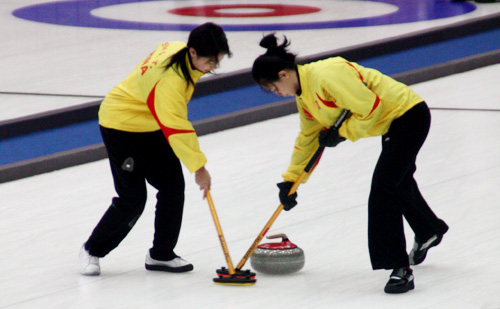
\includegraphics[scale=0.6]{curling.jpg}
\end{figure}

\vignette

或许因为性格内向,我常常在网上的聊天室认识女性,也有不少女孩「上钓」。 有时我觉得,这些女孩独具慧眼,懂得欣赏我的见解,而且她们爱国。 但如果这真人秀不存在,那些女孩根本不谈任何条件,就会在网上免费和你做爱,甚至我是个疯汉也没问题?  我那么辛苦读书、做研究,有区别吗?!

有个香港的大学女生,在电话上谈了一会,便在当晚来我家过夜。 她见到我后有些挑剔,似乎不满意我外表或年龄,我心里开始有些不快,又想起较早前在网上看到的AV片,觉得那AV女孩的表演是在挑釁我,因为她们都知道我是谁.... 越想越想.... 我和那女生躺在床上聊天,她问我我喜欢她吗? 我就晦气地说「普通吧」。 然后第二天早上她说她要走了,我没有挽留。

她走后,我发觉自己很喜欢她,哭得很悲恸,我搞不清为什么她要走,也搞不清是不是因为这臆想病令我说了不该说的话。 几天后我到她读的大学图书馆还书,看见路上的女生有她的影子,路上行人的眼睛红了好像想哭,好像举世都为我而哭了。

我发觉我在网上做爱时,是用没有被监视的那边脑子,而如果一面想著被人监视的话,根本无法做爱。

据说有些野生动物,牠们只会在野外交配,被人类困住之后就不会交配,所以只有例如牛、马、狗等种类能被人类驯养。

但可惜我有时会用另一边脑袋和女孩说话,可能把她们吓跑了....

而且我也察觉到,自己的脸两边越来越不对称,一只眼比较大,眼眉较高,看上去很开心和善良,另一只眼较小,眼眉较低,看上去很凶,像杀人犯。

\begin{figure}[H]
\centering
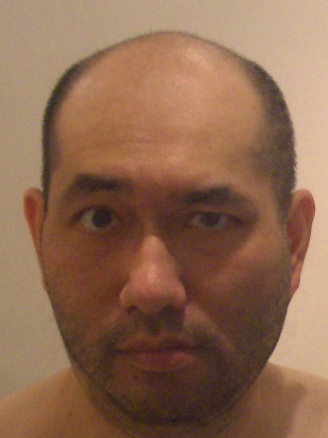
\includegraphics[scale=0.6]{2015June.jpg}
\end{figure}


\chapter{妈妈}

未能去纽约找堂妹前,我在香港想念她,又没有通讯。 那 5 年间我的生活极度抑郁 (depressed),又怪我父母不准我见她 (但其实她也不会想见我)。 我在房内不停写「讨厌」两字,有一天我妈居然在我的涂鸦上写着「何厌之有?」 那更使我讨厌到无以复加。 我很想说:『妈,那就是你呀!』 但那样的话实在难以启齿。 我还未解释: 我自幼便觉得我妈畸恋我,感觉像那电影《Fatal attraction》(但我其实未看过它)。 过了几天,我终於忍不住对她破口大骂,大意是指她不守妇道、我是我、她是她、我不是她占有的、等等。 听我爸说,她那天晚上哭到不能止哭。

自幼,我爸不能驯服我妈,又对我妒忌,因琐事借故拿我出气。 至少我相信是这样。 而我爸做错了什么? 难道他这生有出卖过任何人? .... huh?

但我妈的思想大概没有那么深,她只是说:『这世上人们互相利用,谁都是这样。』 我也不认为她讲得不正确,只是有些浪漫的人不会说得那么露骨,而我喜欢用客观的科学去分析一切。

有一次我们在外国旅行,和一些远亲吃饭,亲戚中有个丧了夫的寡妇,而我妈和她说笑,说什么『老公早点死掉还更开心。』 而我爸坐在旁若无其事地吃饭、付钱。 从小到大,我看见母亲都是这种态度。

有时期常叫我父母离婚,因觉得我爸受蒙骗,是一颗终会瞒不住的计时炸弹。 但有一次争辩中他冲口而说:「我也有个情妇,她也叫 Anna (我妈叫 Anna),你是不是想见见?」 我顿时啼笑皆非,这实在太正常了。

在纽约,我在伯娘家的厨房偷看堂妹的笔记,发现她写了些少女情怀的诗,使我像着了魔那样好奇。 晚上她放学回来, 抢了笔记本然后对我破口大骂。 那天晚上我回到大学宿舍,在床上哭了一晚,一面哭一面自慰了很多次,这生人都未试过那样。

后来,我想忘了她,继续亨利 8 世的计划,但我大概不会再那么爱一个女人了。

而我又想,那些偷看我的人,也应该受到同样的教训.... 如果真有其事的话。

\chapter{打阿妈事件}

入精神病院的直接原因,是因为打阿妈。 话说我很讨厌妈妈买东西给我,例如衣物或日常用品,而她几乎从不买东西给弟弟。 可能是因为弟弟很喜欢高品味的东西,而我比较不修边幅,我这辈子通常都是穿著别人买给我的衣服。 其实是因为我注重环保,而明白到物理学上的物质和能量守恒,令我经常把世界看成是近乎零和游戏那样; 这对於不懂科学的妈妈和弟弟可能很难理解。 好不容易才把一件讨厌的衣服穿烂了,妈妈旋即买一件新的回来。 又,因为我穿那些老土衣服穿厌了,开始把衣服反转来穿,而妈妈竟然买了一件款式是露出线缝在外的 T 恤给我,尺码又紧又不舒服。 还有一次,我看到外国人的笑话,说「如果你....,你就是中国人」, 其中一项是「你把牙膏用到像纸一样扁 。」 我觉得很好笑,於是故意把牙膏压得扁扁的。 谁知妈妈买了一个用卷轴挤压牙膏的工具,还把它卷在我的牙膏上,摆在洗脸台前。 世上有很多人不够衣服和日用品,而我眼白白看着这些物品浪费,简直是折磨。 我已经跟她解释了无数次\footnote{虽然在数学上是有限次},包括那环保理论。

我发觉她根本不是关心我,而是在赌气,因为不想我追到漂亮又聪明的洋妞而变得性格乖戾。 有一次我甚至中英文粗口并用来骂她买东西给我,她说:「噢,你讲粗口,我不跟你谈了....」 然后她又承诺不再买东西给我。

我那时已经是成人,2009 年,38 岁,脸上长了第一根白须。 和家人同住实在太多磨擦,所以妈妈决定给我买间房子。 本来我想买便宜的,为了保存资金作人工智能的创业用途,但妈妈结果买了 3 倍贵的房子,也不用徵询我同意(尽管这投资现在看来是不错的)。 我在看楼的时候发脾气骂她,而我爸说:「我就想到他一定会骂 …」 后来我们去买家俬,我自己选了一张像钢琴形状的黑色桌子,而我从来不懂弹琴,所以那天心情特好。 我用轻松的语调警告我妈「不用给我的房子添东西啊,我自己会买!」 这样叮嘱了 3-4 次。

「热水壶呢? 你一定要煲热水的。」\\
我说:「不要,我想自己选,我也喜欢购物。」\\
「小型的电焗炉。」\\
「不要。」\\
我还向她解释了为什么不用焗炉,因为高温焗东西会产生 AGE (advanced glycation end-products),加速老化。 姑勿论这健康理论正不正确,每个人有权管理自己的健康的,各位读者有没有异议?

记得是一天后(顶多是两天),我下楼看到妈妈已经把我的物品包扎好了准备搬家。 妈妈在楼上,爸爸好像有第六感去了郊外散步或游泳。 我心跳加速,用刀剖开纸皮箱,果然看到那两件东西。

回想起来,一个人买礼物送给我,就算她的动机多么可鄙,我也没有权打她。 事发前我们已经找过社工来排解纷争,那时妈妈辩解说:「母亲爱儿子,有什么不妥?」、「我不爱你爸爱谁?」

其实那也是我想问的: 「妳口口声声说不爱我爸,那妳不爱他爱谁?」

我觉得实情是她后悔以前畸恋我,现在和我斗气。

我拿起焗炉跑上楼,把它狠狠地摔在她房间的墙上,然后掴了她一下,又拿沙发椅子摔向她,并要她跪下来陪不是。 之后我知道脾气暴躁的爸爸回来后必会导致命案,所以我拿了厨房的菜刀,反锁在自己睡房,用床诸塞门口,然后报警。

那些警员是父亲以前的同事,他们都想大事化小。 众人都已归於平静,但我爸坚持要我到医院检查精神有没有问题。 精神科医生要我住院一晚以便观察。 他们和我谈的时候,我天真地想,不如借此机会请教他们我的 paranoia 问题 —— 而的确,我很需要人帮助。 但我得到的「帮助」完全不是那么回事……

自幼,不知是不是母亲的间接暗示,我常喜欢模仿疯癫的行径,母亲大概觉得那是有才华的表现,我也自觉很有意思。 我的同学朋友也知道。 想不到现在真的变了「疯子」,但我惊觉那不是闹着玩的,就像老鼠怕老鼠夹,那疯人院对我而言真的是 booby trap。

为了逃离疯人院,我迫於无奈,在探病时抓着妈妈的手说:「妈,我很疼你.... 快救我出来。」 那就像「芝麻开门」那样有效。

出院后我和妈多了谈话,因为要定期覆诊,要「表现良好」。 我搬进新屋,但不久之后妈妈送的礼物又再像恶梦般回来。 先是 4 只凉衣架 —— 我其实真的不够凉衣架用,但看到那些凉衣架真有欲哭无泪的感觉。 终有一天,我会追到女朋友,逃离她的魔掌,绝不能被 4 只凉衣架搞到性无能。 我向她解释:「新闻说有个痴情男子在餐厅铺满玫瑰向女子求婚,但也被拒绝了。 若他每天送玫瑰,送十年,天天浪费时间和资源,那女孩也不想要,对社会也没贡献,这样做人有什么意思? 我也接受了堂妹不喜欢我的事实…… 我现在连她在地球哪一洲也不知道。」 我妈回答说:「不是的,你不知而已。」 Huh? 难道我堂妹还喜欢我? 已经想了十几年,以为抛却在背后了,究竟还要想多久才有结论?

究竟我妈明知我不想要却坚持要送东西给我的动机是什么? 如果她真的为我好,应不会这样吧? 有时甚至怀疑她老人痴呆症,但她又否认。

我妈不喜欢吃太甜和冻的东西,我想最好每次见面在 7-11 买杯思乐冰 (Slurpee) 给她。 那种东西在整个冬季有没有人按一下都成问题,但又见它不断在搅拌。

在美国时,有一次在堂妹家的后门等她回家,等到深夜,见她的车子开进来,被车头灯照得睁不开眼。 我可怜兮兮地望着她,想博一點同情分。 等她泊车,谁知她是在急速掉头,想避开我; 在那很窄的空间,她驾车技巧的纯熟令人诧异。 人们常说女人驾车「姐手姐脚」,但她们发怒的时候比赛车手还凶。

我明白到,不想要的爱,是会令人感到极度烦厌的。 有次我和堂妹在她家门口纠缠之际,我看见她的眼里也有泪光,但那跟我的眼泪是有着 180\textdegree 相反的意思: 她觉得我可怜,但又不喜欢我,但又被我的苦苦纠缠弄得很痛苦。 为什么被痴缠的人总有那么强的欲望去让痴缠者死心,好像不那样做不行? 但每个月收些不想要的礼物,又真的会逼到人发疯。

我偶然看过 Tom Cruise 到中国做宣传,那些年青的中国女子,多得像人海那样,她们伸长了手臂在召唤偶像,泪流满面、歇斯底里地喊着。 照上面的理论,那傢伙肯定定变性无能了(因为有那么多单恋他的女人)? 但后来又想到,Tom Cruise 是自愿当明星的,那是双方自愿 (consensual) 的偶像-影迷关系。 有天我也想在台上引吭高歌,听台下万千观众的欢呼....

妈喜欢看书和看电影,《红楼梦》、《罪与罚》、《飘》那些书她都从头到尾看过,又怎会是那么笨的人? 她最喜欢的小说是 Jack London 的《海狼》。

在《知乎》网站上看到人们评论一则新闻,说有个无经验的大学小伙子,在女生宿舍楼下求爱,用洋烛摆了 I LOVE YOU 的字样,但那不领情的女生走下来用水盆把洋烛泼熄了,还用盘子扣在男生头上。  类似这样求爱不遂的事件时有发生,我看人们在网上的评论,察觉到很多人是非不分,评论别人时什么离谱的话也说得出来。 如果说那男的做错了,他做错了什么?  如果他纯粹缺乏经验,那女生有什么权打他呢?  这件事就和我打送礼物给我的妈妈一样,只不过男女角色互换了。  但我觉得我妈明知我不喜欢她送礼物却故意送给我,是在挑釁。  而那男生也有可能明知女的已经婉拒了他,却仍然装蒜在跟她斗缠。

%印象中我接触的很多西人,评论事件时态度认真,像写哲学论文,但回想起来他们的混帐言论也很多。 

\chapter{精神病院}

在正式关进精神病院的时候,有男护士要我签字同意治疗,我问他说如果不同意会怎样? 他说就算不同意也会强迫入院,所以没有分别。 后来我出院后到精神病人福利团体那里了解,其实我是有权不接受治疗的。 那些精神科医生很想关病人入院,因为不这样的话他们没有生意,他们收入的来源其中一部分可能是由美国的药厂赞助的。 精神科药物为美国经济带来每年很多亿元的收入。 他们找个低级的护士迫我签字,那样便毋须负责任。

医院里光怪陆离,像动物园,如果不是没有自由,那会是个很有趣的地方。 有个来自大陆的年青人,他说「我妈不知给我喝了些什么汤,喝后会使周围的人知道我在想什么。」 我说话开导了他一下,但那时我也自身难保。 其实他的病和我的病一样,但我受过科学的教育,不会迷信,我的病以不违反科学的形式呈现出来。 他整天听家人给他的收音机,学广东话。 那令我想起,香港人普遍歧视大陆人,就像美国很多人歧视我们华人一样。 我和他都感受到周围的人的敌意,产生了逼害臆想。

病友中还包括:
\begin{itemize}
\item 一个因前妻外遇而自杀过的中年人,要吃开心药。 他很健谈,常对我们讲历史;
\item 另一个因妻子不忠而拿了菜刀和她吵架的人;
\item 一个读数学的大学毕业生,他幻听的声音常叫他做一些不明所以的事,例如丢掉某些东西;
\item 一个中学高材生,用刀割过自己的手腕,拉起袖子让我看很多条刀痕。 他说他当时像神志不清那样,不知为什么那样做。 我和他下棋,输了给他。 我向他解释神经末梢的原理(neuron、axon、dendrite、synapse 那些),建议他不要吃药,第二天他就不见了,不知是回家还是调到另一病房。
\item 一个在便利店偷东西的人,他说他自己也不知道为什么偷了几本杂志。 吃了药的他手震得很厉害。
\item 还有几个是「长期住客」,据说他们被困在细小的病房里有很多年之久。 我们病房大约两间中学课室那么大的地方,这样被长期监禁着,是很不人道的。
\item 一个在晚上会叫你「早晨」的人,但他其实也像正常人,只是很爱开玩笑。
\item 还有一个不会说话,样子像怪兽、叫声也像怪兽的怪物。 他有没有受医护人员虐待都很难说。
\end{itemize}

看过 YouTube 上外国女孩把自己在精神病院的片段登上去,我在想:怎么她们那地方像 Hotel California,而我们这里像 Iron Maiden?

覆诊的时候见过一个年青人,面色苍白,手震得很厉害,像那些心脏衰竭的老人。 那是很典型的药物反应。 我心想,他被药物弄成这样,必早死,就算将来减少剂量,他的寿命也会被弄短好几年。 这些医生简直是在慢性杀人....

如果明白那些药的作用,根本没有人会肯吃。 美国的药厂隐瞒事实,把「毒药」输送到亚洲,而亚洲的行政人员对他们唯命是从,毒害了无数的无辜的人(虽然在数学上是有限)。 然而,美国或西方的没落,其规模之大可能还远远超过这样。

和那中学生下棋的时候,有个男护士走过来,看了几秒便对我说:「你在两步后会有危机。」 我看不出来,甚至在他告诉我以后,我还要下两步棋,然后才发现对方马后炮。 据说孙中山下棋也不高明,爱急攻,但忽略防守。 但奇怪的是我下国际象棋时认真很多,虽不算是 master,但也攻守兼备而且很「靠谱」。 我有个理论: 在中学时那些喜欢国际象棋的同学,比较有国际视野,而喜欢中国象棋的人会倾向留在香港或中国发展。

\chapter{发病的原因}

1996 年我初到美国,心里像尼采所说的『这杯子将再度变空』,我要虚心学习,目标是要青出於蓝。 我对美国人没有恶意,我要胸无城府那样接待他们,而且要为中国人争光,不要失礼。

很快地,我发觉我无论做什么,都好像变成了美国人的笑柄。 我写了一封情信给堂妹,信封上画了我抱著她的画面,那幅画抄袭日本恐怖漫画的美女,她的头发像波斯湾里漆黑的石油涌进大海\footnote{这个比喻是一个美国女作家的,忘了出处}。 内容大意说: 我来了,在 Long Island 的这间大学,我很挂念妳。 但她见到我后似乎非常厌恶,好像我在她身旁很失礼她。

我穿的衣服、行为举止,都有点格格不入,而且年龄比普通学生大一点,觉得自己在课室里很惹人注意。 而且很奇怪地,那些美国女生不断对我抛媚眼,她们 come-on 的大胆程度,即使我思想算很开放,也令我很惊讶。

我逐渐留意到一些巧合的事,例如我在宿舍房间内做的事,很奇怪地变成了教授开玩笑的话题。 於是我怀疑有些学生在故意恶作剧搞我,因为美国大学常有恶搞新生的事件,而这传统在香港没有那么极端。

当我开始有被偷窥的想法之后,我做了一件(我自己觉得是)很惊人的事,就是我「将计就计」地把自己的私隐公开出去,目的是要向全世界揭发我认为是欺骗人的事。  例如我觉得我堂妹在骗我感情,我妈欺骗我爸感情,还有美国的虚伪,他们假装和我开玩笑其实是想整我,因为他们知道我会是帝国的终结者,我的成就终有一天会盖过他们。 那是真的: 我真的有那样的抱负。

我在美国写电邮给在香港的前度女友,和她报告我在美国的所见所闻,有时也哭诉堂妹如何令我心碎(我就是因为堂妹所以和前度分了手)。  她没有到过美国,我说的故事令她很感兴趣。  但我在写给她的电邮里,故意暴露很多真实的事和心底的话,而且尽量写得诚实,因为我知道我的偷窥者们一定会看得津津有味,这种真人的「演出」比所有电视那些经过彩排的假故事一定更吸引。  而当他们将我的趣事一传十、十传百那样传开去,最后帝国的谎言就会像「国王的新衣」那样人尽皆知。

这个计划似乎很完美,可惜有个漏洞: 就是我自己也无法肯定究竟有没有人在偷窥我。 当我开始想验证的时候,我发觉这件事简直不可思议地\ds{无法验证}。  所有巧合的事,都可以解释成真人秀的存在,也可以解释成巧合。

有些逼害臆想症的男人老是怀疑自己的妻子红杏出墙,即使妻子很忠贞也是如此。 但我质疑这究竟算不算是一种病? 当然,如果妳就是妻子,妳当然知道自己有没有和别人睡,但妳又怎能假设正在外面上班的丈夫知道妳私下做什么?  如果他不知道,他就有怀疑的理由,这不是很科学的态度吗?  而且这世上的确有很多红杏出墙的妻子,我在网上也和她们玩。

\begin{comment}
我和初恋女友常常因为我的怀疑和猜忌闹得很不快,但我一厢情愿地信我堂妹爱我,其实她早已不喜欢我,我白白等了她很多年,觉得这种专一的游戏很幼稚,浪费时间在互相猜忌。
\end{comment}

有了被人監視的想法令我在美国每天的生活仿如人间地狱。  扭开电视,看到有科幻片叫《星际笨蛋》\footnote{Inter-galactic Idiot},我以为他们在嘲笑我。  无他,因为他们必须永远假装在开玩笑,否则便要面对老实地谈判。  我初时常常觉得美国人的幽默很好笑,但越来越觉得他们笑里藏刀,是一种恶意地贬低别人的心理战术。

终於毕业,回到香港,我在行李箱内放了我以前写给前度女友的所有电邮(每次写完比较长的电邮就用学校的打印机印出来),那是重要的记忆,作为日后参考之用。 我在香港待了约一年后,突然有一天怎样找也找不到那些信件。 问我妈,她的表情天真得像个 13 岁小女孩,她说:『噢!我丢掉了。』

她不是蠢,而是占有欲很强,把儿子当做一件附属的东西。  这不是她唯一一次想毁掉我的记忆; 第二次是在精神病院里,如果我不机警,那些精神药已经令我变了傻子。

如果不是写这篇自传,我差点把这件事忘了。  现在我很愤怒,我不是想打阿妈; 我简直想杀了她。 

我看过一本英国女人写的自传,她少女时被父亲性侵,他还约朋友到家里把她按在床上轮奸。 后来她离家出走,找到了肯爱护她的男人。 我自己也是个好色男人,有时喜欢扮 daddy 和女孩玩幻想的轮奸游戏,看到她这样厌恶父亲,不免感到有点「没趣」,但当然她是对的。  也听说过有些父亲和女儿变成了情人关系,我觉得只要是双方自愿的,那样也没有什么不妥。

不时看到很多歌颂母爱的电影,令我非常厌恶,我觉得他们故意站在我妈那边。 我妈假装她爱我,其实我要揭发的人,其中之一就是她。  她假装骗我是为了我好,因为如果不骗我的话,美国那边会派人杀了我。 但其实美国政府已经处於劣势,他们想为所欲为也有制肘。 我妈和某些香港人、中国人,他们妒忌我计划的成功,故意将美国说成很强大,作为他们出卖中国人的借口,继续骗我。

\chapter{和堂妹相似的人}

最近事情又有了新发展:  接近 100 岁的嫲嫲生日,我们一班亲戚在酒家吃饭。  席间, 冷不防表姊提起要打长途电话给堂妹们让她们道贺。  我听错了以为她们又来了香港探亲,要上来酒家,突然间我的面容很可怕地扭曲起来,像是突然遇到多年不见的仇人,过了整整 3 秒才 regained composure。 我觉得表姐们一定看见了,而她们都知道我和堂妹的瓜葛。  我也很奇怪,明明觉得自己想通了,现在已经很释怀,和其他女人玩得很开心,但原来心理上还是留下了很可怕的阴影。

表姊们传递手机上的照片给我看,我看不到堂妹,但看见她新近结婚生下来的BB。 那婴儿房的布置,整间房间都铺满了老虎的毛毛玩具,俗不可耐。 我暗付:『好彩当年追不到她。』  过后又想起: 她还是没变,还是像老虎那样凶,动不动就想打人。

又过了一两年,在网上居然发现了她的 Facebook,我看到她的老公是个白人,样子端庄,还算给人好感吧。 可是我看着他们来香港旅行的照片,怎样也感觉不到一丝快乐。 我身边的新女友说:『他们看上去很快乐啊。』  『是吗?』

又传来她儿子的相片,那小孩子一头金发,身上完全看不到一丁点中国人的特徵。 我堂妹应该感到很欣慰了吧?

听亲戚们说,她很喜欢游泳、潜水。  我怀疑她还记不记得起布殊喜欢打高尔夫球....?

回想起来,我堂妹很不喜欢说话,可能是因为我们言语不通,她说的中文很有限,而我又很爱面子地不肯在她面前说英语。 在纽约那段日子,我能够记得起她说的话,就只有一些单字,她就像个白痴那样只会说单字,但又好像想用那些单字来迂回曲折地暗示些什么。 我们一起吃晚饭,她和我妈谈到在美国的商店买货品,凭单据可以无条件退钱或换货品(香港人会觉得很惊讶)。 然后她突然煞有介事地说:『\ds{交换}嗱!』用的发音有点偏差的广东话。 在送我往机场的路上,她指著机场附近的人说:『噢,有那么多\ds{中国人}!』  我堂妹真是全球说话最拐弯抹角的人。

她姊姊说话比较直接:『你觉得我妹妹在 egg you on, right?  你是不是觉得我们在\ds{出卖}你呀?』  我被气得对她姊姊破口大骂,但她姊姊狰狞地说:『噢\textasciitilde\textasciitilde 我们很害怕呀\textasciitilde\textasciitilde ~!』

其后我常常思量堂妹说的「交换」的意思。 我在网上结识很多白人女孩,处处在她们中间寻找堂妹的影子,但仍没有人和她太相似。 直到我放弃了找白人女友,我开始约会一个中国女孩。 我已经忘记了「交换」。

\vignette

那中国女孩身材有点矮矮胖胖的,和我堂妹一样(也和我妈一样),但我初时没有联想起来。

我们在散步,地上有一块「小心地滑」的牌,她看了后侧著身轻轻地滑了几下,说是『小心地 ~滑』。 那姿势令我想起堂妹跳蹦蹦时也是这个模样。

在餐厅她点了红豆冰,她说她喜欢红豆,但不喜欢冰冻的东西。  我突然记起我妈也喜欢红豆,她也不喜欢冰冻的东西....

我和她的关系急转直下,差不多为每件小事都意见不合。 她做错了事从来不\ds{道歉},而且觉得自己永远是对的。 她说话很特别,在5分钟内可以前后矛盾。  我记得14岁时的堂妹也是这样,令我感觉奇特,但我已记不起她当时说的什么话题。  堂妹14岁时常常无情地批评我,我那时觉得她身体是个小女孩,心灵却是1000岁的精灵。  现在面对这个「堂妹2号」,她虽然已经27岁了,我觉得她竟蠢得像1000年未用过脑那样。% 又想起我妈,我觉得她简直生来就是老人痴呆症的。

我很喜欢村上春树的比喻:「一切都像描图纸那样错开了....」

好几次看到她在哭,因为我不喜欢她了。  我的心隐约感受到记忆中很久以前的痛,因为她就是以前的我。 我想对待她好一点,尽量做得和堂妹对待我不同一点,因为我要证明堂妹那样对我是错的。 我很耐心地将一切解释给她听,甚至这份自传也是写给她看的\footnote{或者说想写给我将来会认识的所有女孩},但她说她不像我堂妹(她似乎无论我说什么她也持相反意见)。 我很愤怒,觉得她不可理喻,语言好像对她失去了效用。

我故意开导她,令她不再犯我当年犯的错误,但她就像一个考全A的女生,将所有功课交齐: 我以前对堂妹所做的每一件卑劣的事,她像有只第三眼那样回赠给我,真令我感到「天网恢恢,疏而不漏」。 有一次我在纽约的唐人街买了一盒人参给她们, 因为我觉得人参是中国特产,可以令堂妹想起我们本是同根生,而且我记得妈妈小时候对我说,有些人参生长得像人形,濒死的病人吃了也可以起死回生,令我觉得很神秘。 我送了给她们,她姊姊对我说:『谢谢你啊,这人参含有 stimulant,吃了感觉精神很多。』  其实她婉委的意思是说,不要迷信人参是神奇的药,它只是含有一些化学成份。

其实所有「初到贵境」的美国华侨,都要经历过这些学习,每年成千上万的新移民经历著同样的事,

我真的觉得呼吸困难。

我不想打她,因为我要做得比堂妹更好。  但她的荒谬行径和说话,好几次令我想狠狠地掴她,想用尽全力地用腿将她撑开,让她飞撞到床外的电视机上。  我最终没有打她,但已经愤怒得身体在发抖。  我又想起来了.... 「有些女人就是喜欢将男人激到发怒....」

我反锁上门,在睡房里哭了....

「交换」是假的.... 她两次都不喜欢我....

我警惕自己,她们是两个不同的人,不应该混淆了,但感觉上真的像被同一个人抛弃了两次。

(以下的几章是草稿,日后还会增补....)

\begin{comment}
我本身在政治上經常批評美國,但我自己也曾在美國留學,當然美國學歷令我在香港有點高人一等,而且我爸甚至是英國殖民時期的警司,他的錢可以說是為殖民主義服務而賺的。

問題是很多香港人憎厭我(似乎是這樣),但他們自己也變成了親英美的人。 我覺得他們不能要求我先「償還」然後再反美,因為這樣我根本不能生存。 但我已經說了會為自己過去的特權給他們補償(況且當初變節的人是我爸,不是我),那麼責任似乎就是在他們身上,他們應接受我的意見。

很多人就是太挑剔,什么也不肯妥协,其实在不妥协的过程中,他们自己本身也犯错了。 必需要成熟起来的。
\end{comment}


\chapter{爸爸}

(....)



\chapter{人工智能}

较年轻时的 Ben Goertzel:
\begin{figure}[H]
\centering

\includegraphics[scale=2.0]{benbenben.jpg}
\end{figure}

\chapter{种族主义}

谈谈关於种族歧视 (racism) 的问题。 有很多人似乎不明白什么叫种族歧视。 如果一个中国女孩的 9 个男友都是白人,我们不能强制她第 10 个男友一定要是中国人。 我们吃其他动物的肉,因为牠们比人类蠢;因为我们可以这样 (``because we can'')。 那么说,白人的餐馆不准黑人进场、在巴士上有不准黑人座的位子、分开黑人和白人喝的泉水机,那都是合理的?

纳粹德国逼害犹太人,使大量的犹太科学家移民到收容他们的美国,而 Manhattan project (制造原子弹的计划) 中几乎全是犹太的科学家。 从此美国人和犹太人之间有了互利的关系; 美国人大概潜意识地相信,只要讨好犹太人便可以像二战时那样「胜利」。

讽刺的是,我遇见的两个美国犹太的 AI 研究者,他们都明显歧视和排斥我。 时移世易,角色好像调换了。 但在我不断责骂他们好几年后, 最近他们态度好像收敛不少。

受过南北战争和二战洗礼的美国人,他们都很警惕不要踩到种族歧视的地雷。 在美国电台错口说了 "nigger" 这字都会被开除。 但其实美国仍然是种族歧视的国家,每天都以种族为理由的战争在杀人。 有些人甚至觉得种族歧视才是对的、跨种族的婚姻是错的,等等。

你可能会问,既然谈恋爱和结婚有自由,为什么人们不能「自由地」组织国家和企业,去排斥其他民族? 但我个人觉得在商业上和政治上的种族主义是「错」的。

问题又回到毛泽东说的「无法无天」才是对的答案。 意即:我们都有自由建立种族歧视的国家、开种族歧视的餐馆、等,关键是我们的「企业」要不断和别人竞争。 国家也是企业,国与国也不断要打仗;所谓「经济就是和平时期的战争之延续 (peace is the continuation of war by other means)」。 所以,曹操的诗结尾说「周公吐哺,天下归心」(周公善待天下贤士)。 因为打仗的人都知道「用人唯材 (meritocracy)」的重要性,而不是「用人唯亲 (nepotism)」。 据说蒋介石就是那样失了民心。

\chapter{结论: 历史发展的规律}

有时心灰意冷,为什么打这场种族解放战那么辛苦? Homer Simpson 说过:如果一件事太辛苦,通常不值得做的。 会不会我的民族真的是狗民族? 为什么那么多香港人热烈地想投向白人的怀抱,不觉羞耻? 最近又看到电视上有香港人说:『就算你駡我是狗,我也不在意。』

有两种 racist 的人: racist 的白人是既得利益者,他们只需靠自己的血统便可以在竞争中获利。 在商业上,如果白人受待遇较好、或取缔能力相当的人而被雇用,那就是种族歧视。 第二类是那些很想做狗的中国人,不惜出卖自己的民族,因为他们已经痛苦到做不做狗都没有分别。 但他们并非真的到了穷途末路; 他们痛苦的原因是因为妒忌那些比他们早「变成人」的人,例如我。 用数学公式表示:
$$ \mbox{我} : \mbox{堂妹} = \mbox{香港人} : \mbox{我。} $$

但我们的民族不能永远为了妒忌而把别人拉下去,否则我们真的会变狗民族了。

现在的策略是: 我会帮助中国人变有钱,但他们要帮我战胜那些 racists。 不这样交易的话,实在不能动弹。

我已说过,堂妹并没有对我做过大逆不道的事;她完全可以拒绝我的。 而我那时的伤痛,可能不是因为她,而是香港和美国文化之间存在的不平等的差异 (differential)。 我们不过是漂浮在文明传播的波动方程 (wave equation of the dynamics of civilizations) 中的一些点。 旧的帝国被新的帝国取代,在不公平的表面下有着绝对的公平。 关於文化和技术的历史进程 ,可以看看 Jared Diamond 的书《Guns, germs and steel\footnote{(1997)}》。

想说的大概就那么多,其馀都是细节而已。

还有,我所讲的「世界 A 和世界 B」,其实差不多是同一个世界,亦即你和我活在其中的世界。 疯人院外面和里面的人没有分别。 我们每天都活在种族歧视之中、每天都互相出卖。 假设我在真人骚里而懵然不知,也不会有人道破这谎言。 他们只会对白人低着头「饶命啊大人」那个样子。 你们就是那些演员。

圣经里,摩西想带以色列人走出埃及,但初时人们反对他,说什么「我们现在做奴隶做得好好的,为什么要走?」 在《Waiting for Godot\footnote{等待果陀 (1953)}》剧里有个人像只狗那样被人用绳索拖着四脚走动,主角想解开他反被他咬。 据说 Che Guevara\footnote{(1928-1967)}帮助非洲人打游击战,被当地士兵的散漫态度弄到心力交瘁; Byron\footnote{(1788-1824)}也试图帮助希腊独立战争,因军队的士气低落而过劳致死。 那个叫「耶稣」的人,也是在类似的情况下被人出卖而死的。 还有太多这样的例子.... ( ? )

我常想起耶稣钉十字架时身旁的两个小偷,他们说『你既然是神的儿子,为什么落得和我们一样下场?』 我的目的就是要不死。

{\color{blue}\hrulefill \raisebox{-4pt}[10pt][10pt]{\,\,\S} \hrulefill}

( Experience with white girls online.... )

%\chapter*{Appendix: XXXX}

\chapter*{Acknowledgments}

( Apologize to relatives and friends.... )

%\bibliographystyle{plain} % or number or aaai ...
%\bibliography{AGI-book}

\onecolumn

% Bigger figures

\end{document}
